\section {Problemática}
\label{sec:problematica}

No ano de 2023 o Brasil Participativo acumulou um milhão e quatrocentos mil usuários únicos durante a execução do PPA.
O alto volume de acesso de usuários e dados utilizados no período resultou na exibição dos primeiros problemas de desempenho da plataforma, que foram observados pelos usuários através da indisponibilidade do serviço durante a situação de alta demanda.

Após os incidentes de indisponibilidade, a empresa responsável pela infraestrutura da aplicação no ambiente produtivo, a Dataprev, conduziu uma análise utilizando dos registros das ferramentas de observabilidade adotadas no sistema.
Em contato direto com a equipe de desenvolvimento do Lab Livre pelo canal de comunicação do Telegram, eles disponibilizaram um relatório indicando alguns dos problemas da aplicação e suas possíveis soluções.

Os problemas listados foram: sobreutilização do banco de dados e a indisponibilidade do mesmo, falta do uso de índices, \textit{memory leak} e lentidão em páginas específicas. Cada um deles será discutido em mais detalhes a seguir.

\subsection{Sobreutilização do Banco de Dados e Indisponibilidade}

O acesso a páginas de propostas e criação de novos usuários gera enorme utilização do banco de dados.
Por exemplo, um dos problemas notados foi o uso do comando SQL \texttt{ILIKE} para desambiguação de \textit{nicknames} na plataforma, que ocorre durante o envio de informações para efetuação do cadastro na plataforma.
Foi constatado que o \texttt{ILIKE} requer bastante processamento do banco de dados, atingindo tempos na casa de dois segundos.

Requisições que demandam tanto tempo do banco de dados, aliadas à alta demanda de usuários, fizeram com que o PostgreSQL atingisse o limite de conexões em seu \textit{pool} em vários momentos.
No ambiente produtivo, o tempo de espera limite para obtenção de uma conexão do \textit{pool} do banco de dados é de cinco segundos, porém diversas requisições retornaram com erro para os usuários por exceder esse tempo limite.

\subsection{Ausência do Uso de Índices em Consultas Ofensoras na Plataforma}

As sete principais consultas mais ofensoras da plataforma poderiam ter seu desempenho melhorado através do uso de índices em suas tabelas no banco de dados.
Através da observação do uso da plataforma no ano de 2023, um padrão de consultas recorrentes foi observado.
A Dataprev iniciou um trabalho interno para implementação dos índices no banco de dados do ambiente produtivo.
A criação desses índices pode ser proposta para a comunidade \textit{Decidim} posteriormente, com o intuito de torná-la padrão no projeto.

\subsection{Memory Leak do Processo Ruby}

Com o passar do tempo, a memória alocada para a execução da aplicação \textit{Rails} aumenta sem dar qualquer indício de recuo, o que implicou em um trabalho extra por parte da equipe de infraestrutura para reiniciar a aplicação sempre que ela atingisse uma determinada quantidade de uso de memória.

\subsection{Lentidão em Páginas sob Condições Específicas}

Durante a navegação pelas páginas da plataforma, foi notada lentidão em algumas delas.
Essa lentidão ocorria na escala de segundos, e em casos mais graves na escala de minutos.
Notavelmente, algumas das páginas que demonstraram baixo desempenho foram: a exibição de propostas com um alto número de comentários, e a exibição de textos participativos que possuíam algumas centenas de parágrafos em sua composição.

Uma das evidências fornecidas pode ser vista na Figura \ref{fig:report-data-prev-comments-elastic-apm}.
Ela demonstra o desempenho da controladora de comentários da aplicação.
A ferramenta utilizada para síntese dessa informação foi o Elastic APM.
Contudo, o problema não teve sua causa raiz diagnosticada.

\begin{figure}[htbp]
  \centering
  \caption{Relatório da controladora de comentários gerado pelo Elastic APM}
  \label{fig:report-data-prev-comments-elastic-apm}
  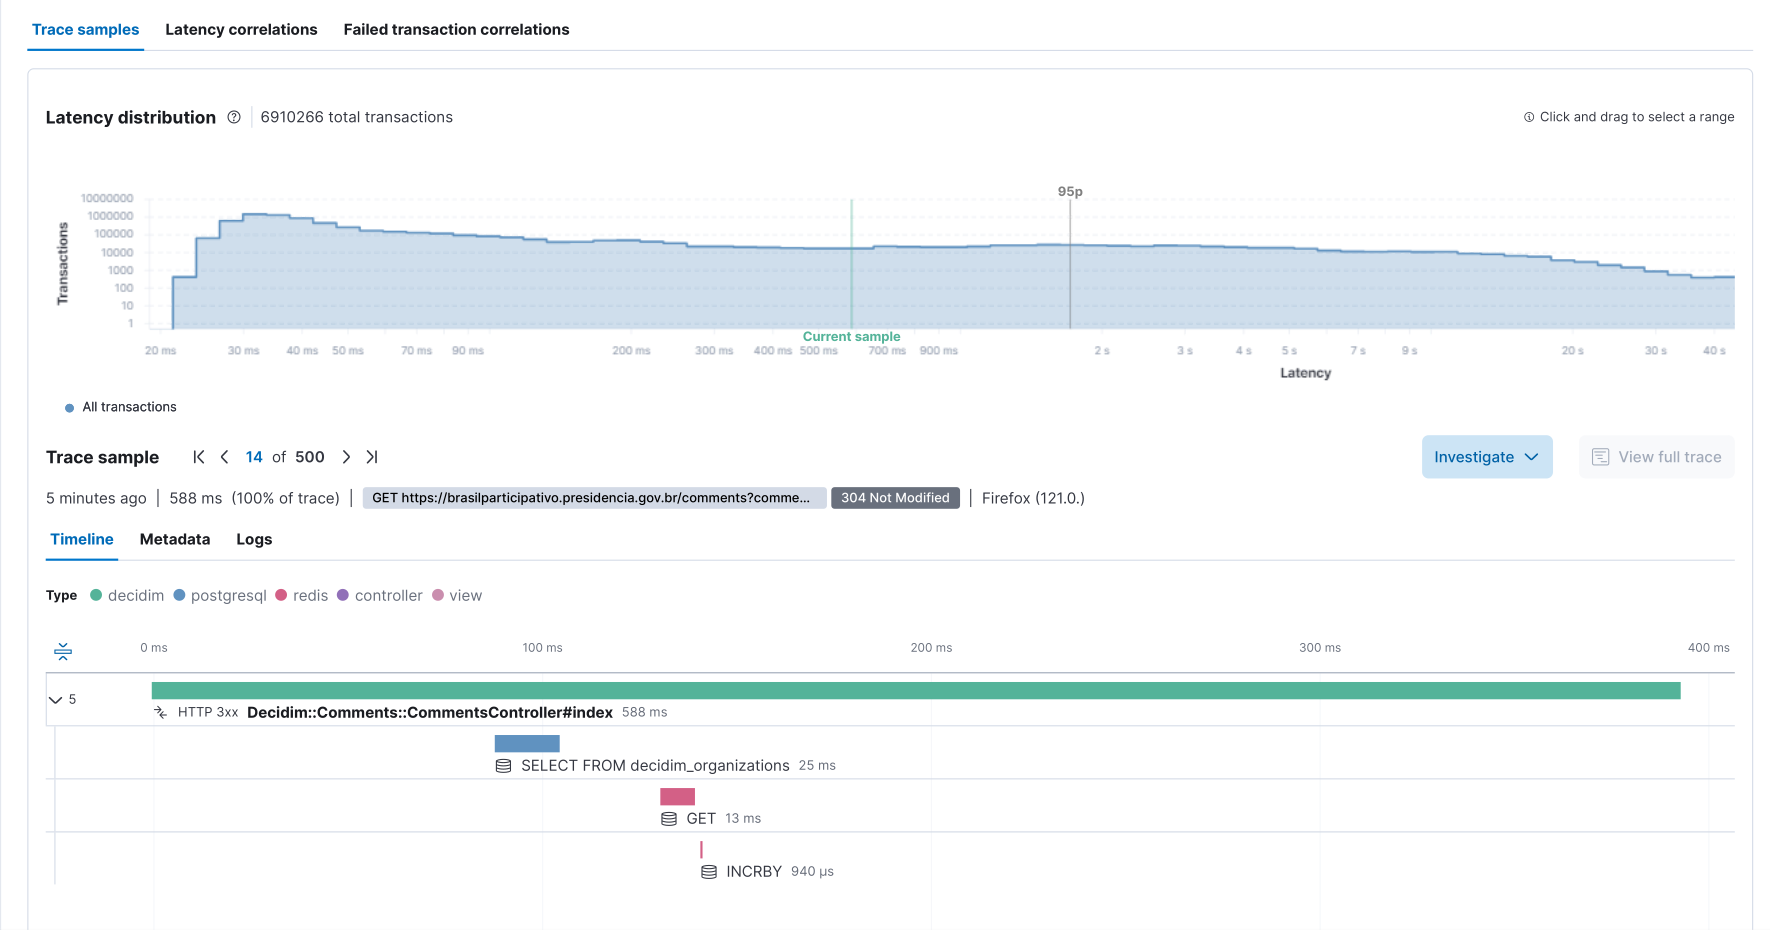
\includegraphics[width=\textwidth]{figuras/report-data-prev-comments-elastic-apm.png}
  \fonte{Dataprev}
\end{figure}
